\section{Saisie des consommations et gestion des anomalies}

\subsection{Fonctionnalités}

Le module de consommation permet au client de saisir les index de son compteur d'eau et de son compteur électrique, de téléverser les photos des compteurs et de consulter l'historique de ses relevés. Il assure également la détection des anomalies et le flux de confirmation ou de correction avant la génération de la facture.

La figure~\ref{fig:sequence} présente le scénario principal de saisie, de détection d'anomalie et de génération de la facture.

\begin{figure}[htbp]
  \centering
  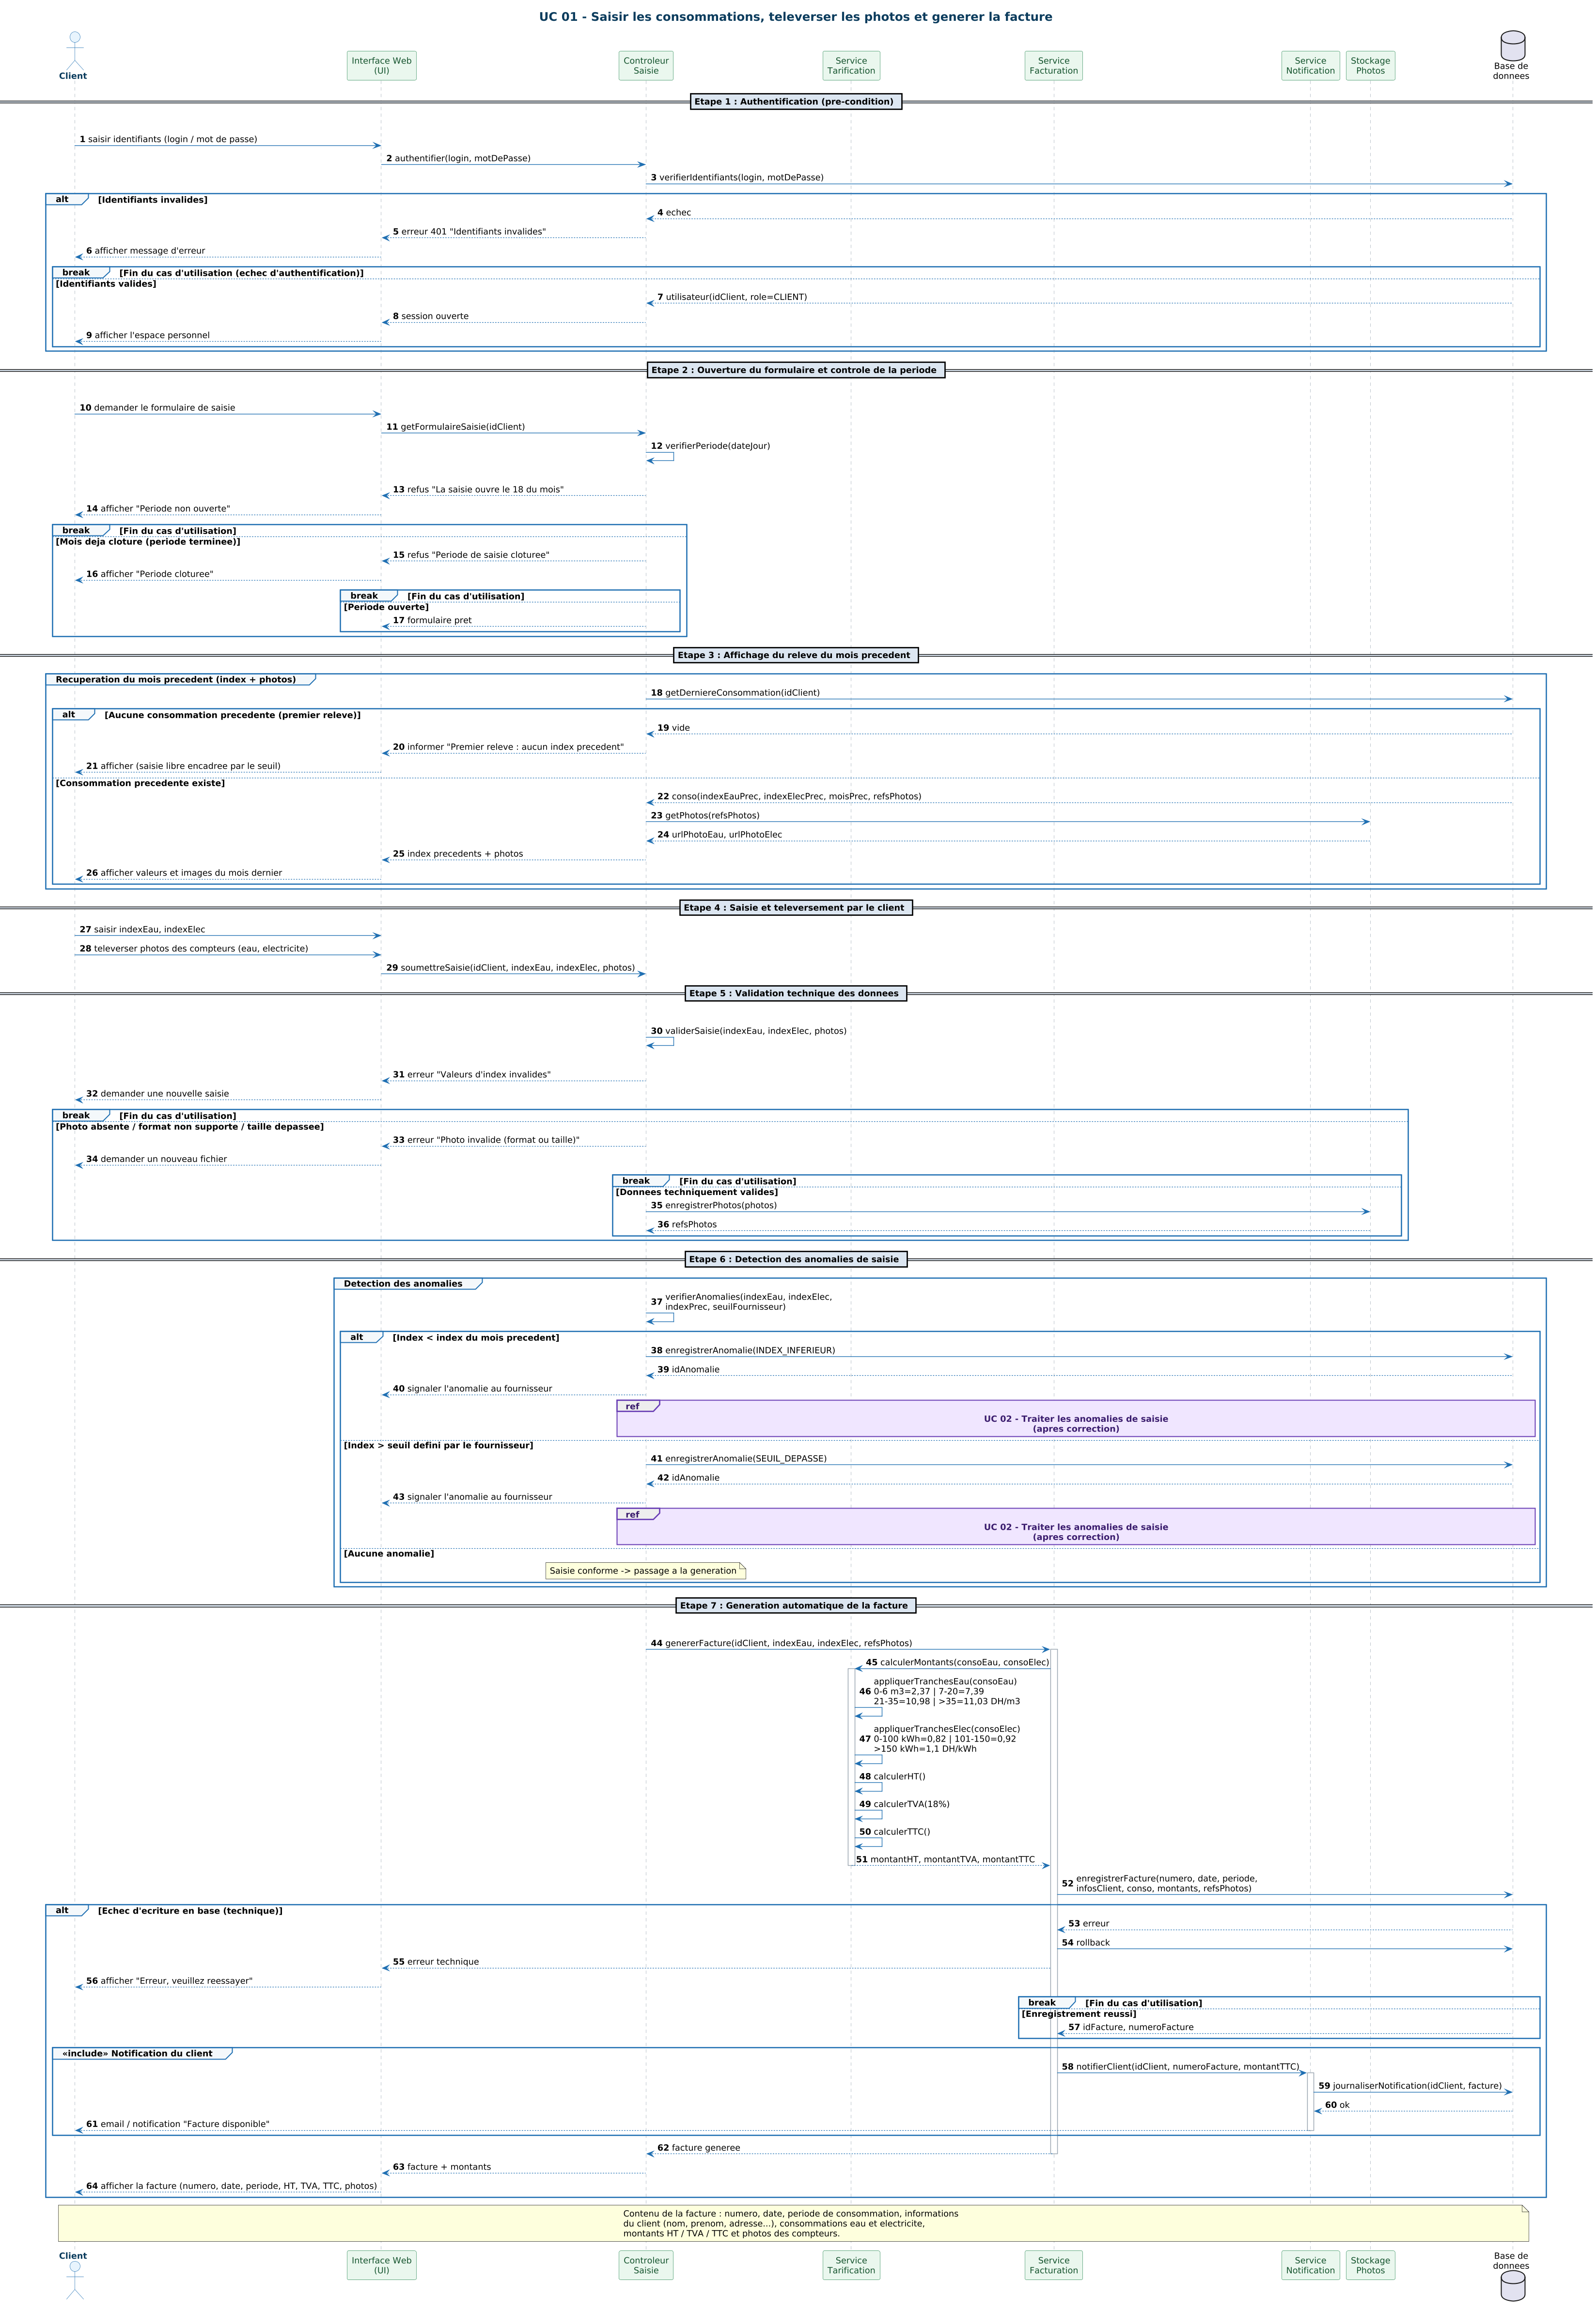
\includegraphics[width=0.60\textwidth]{../conception/diagrams/png/01_saisie_consommation.png}
  \caption{Diagramme de séquence de la saisie d'une consommation}
  \label{fig:sequence}
\end{figure}

\subsection{Période de saisie}

La saisie est autorisée du 18 du mois jusqu'au dernier jour du mois. Le contrôleur vérifie que la période correspond au mois en cours et que le jour courant est supérieur ou égal à 18. Une saisie hors période est refusée avec un message explicite.

\subsection{Formulaire et photos}

Le formulaire présente deux cartes : une pour le compteur d'eau et une pour le compteur électrique. Pour chaque compteur, le client saisit le nouvel index et téléverse une photo. Les photos du mois précédent sont affichées lorsqu'elles existent.

\begin{figure}[htbp]
  \centering
  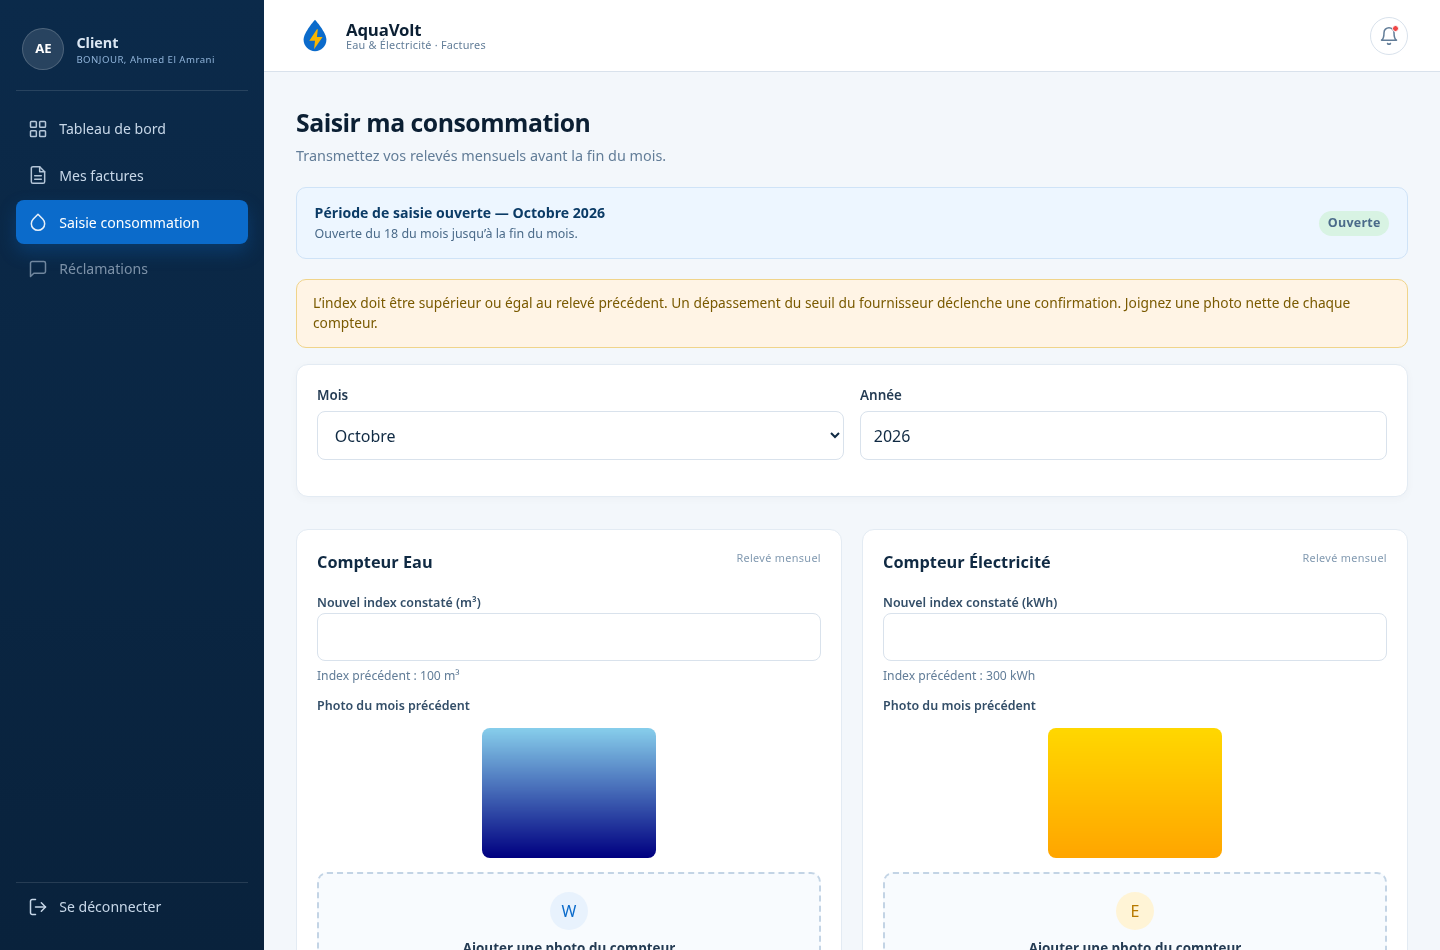
\includegraphics[width=0.60\textwidth]{figures/consommation_saisie.png}
  \caption{Formulaire de saisie avec relevé précédent et photos}
  \label{fig:consommation}
\end{figure}

Les fichiers sont contrôlés avant enregistrement :

\begin{itemize}[leftmargin=*]
  \item présence des deux photos ;
  \item taille maximale de 5 Mo par photo ;
  \item formats acceptés : JPG, PNG et WEBP ;
  \item vérification du type MIME réel avec \texttt{finfo} ;
  \item génération d'un nom de fichier aléatoire ;
  \item stockage dans \texttt{uploads/compteurs/}.
\end{itemize}

Lors d'une correction, les photos existantes sont conservées si le client n'en téléverse pas de nouvelles.

\subsection{Calcul de la consommation}

La consommation est calculée par différence entre l'index courant et le dernier index validé ou facturé :

\[
C = I_{\text{actuel}} - I_{\text{précédent}}
\]

Si aucun relevé précédent n'existe, l'index de référence est zéro. La consommation d'eau est exprimée en m\textsuperscript{3} et celle d'électricité en kWh.

\subsection{Détection des anomalies}

Deux types d'anomalies sont détectés :

\begin{itemize}[leftmargin=*]
  \item \texttt{INDEX\_INFERIEUR} : l'index courant est inférieur à l'index précédent ;
  \item \texttt{SEUIL\_DEPASSE} : l'index courant dépasse le seuil défini par le fournisseur.
\end{itemize}

Le seuil est celui enregistré dans la table \texttt{fournisseur} : \texttt{seuil\_eau} pour l'eau et \texttt{seuil\_elec} pour l'électricité. La règle des +40 \% présente dans certaines maquettes n'est pas retenue dans la version Alpha.

\subsection{Confirmation et correction}

Le traitement dépend du type d'anomalie :

\begin{itemize}[leftmargin=*]
  \item un \texttt{INDEX\_INFERIEUR} doit obligatoirement être corrigé ;
  \item un \texttt{SEUIL\_DEPASSE} peut être confirmé ou corrigé par le client ;
  \item après confirmation, l'anomalie passe à l'état \texttt{CONFIRMEE} et la consommation à \texttt{VALIDEE} ;
  \item après correction, l'ancienne anomalie passe à l'état \texttt{CORRIGEE}, puis le relevé est contrôlé à nouveau ;
  \item après validation, la facture est générée automatiquement.
\end{itemize}

\begin{figure}[htbp]
  \centering
  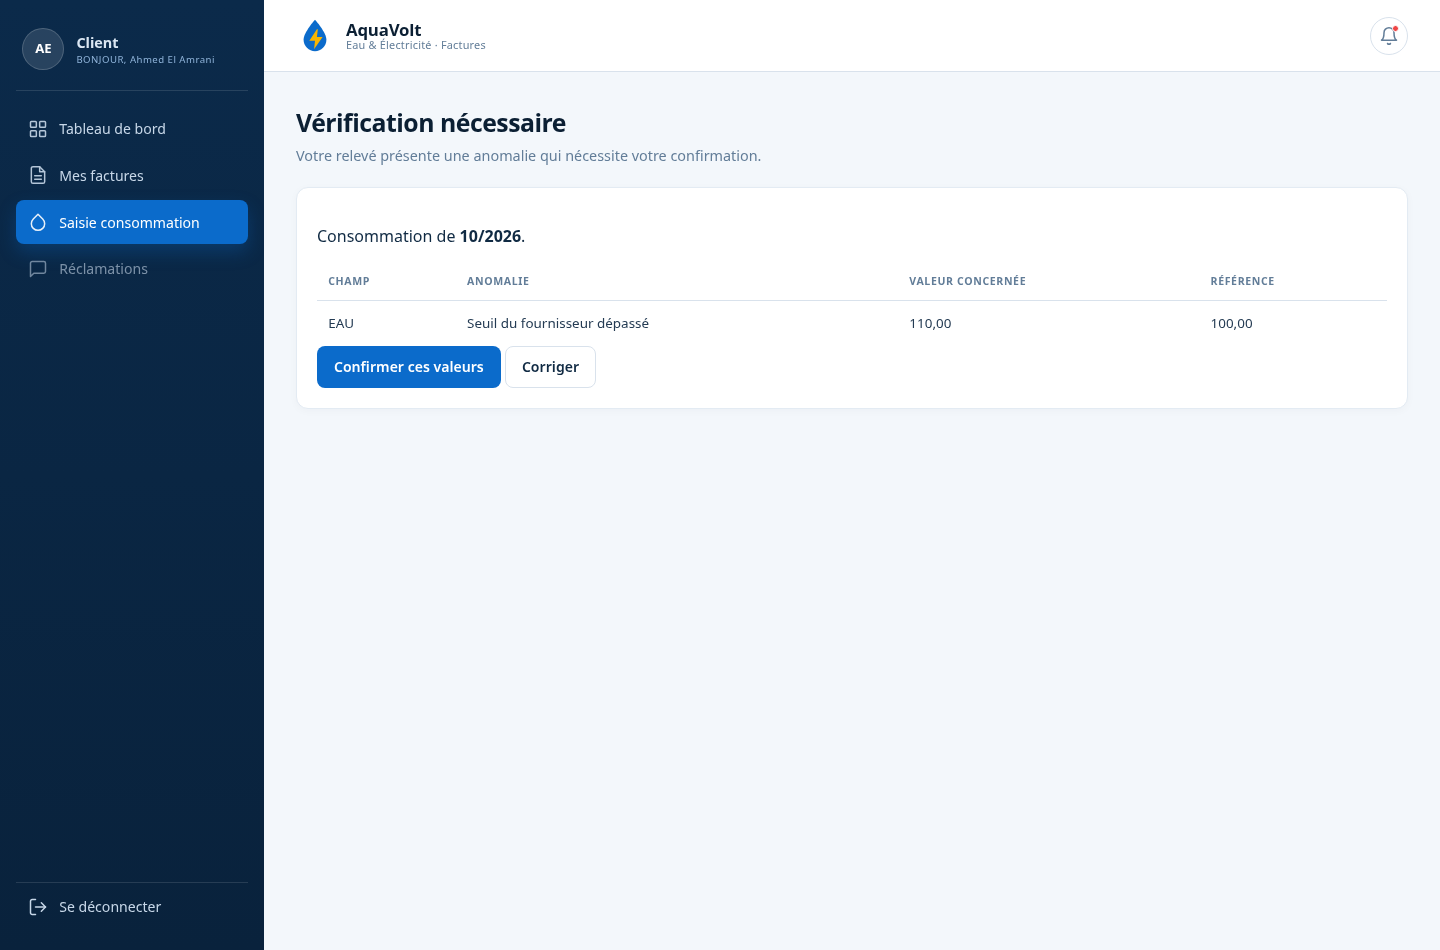
\includegraphics[width=0.72\textwidth]{figures/anomalie_confirmation.png}
  \caption{Confirmation d'une anomalie de seuil}
  \label{fig:anomalie}
\end{figure}

Le fournisseur consulte les anomalies en attente, mais la correction est réalisée par le client dans le flux de la version Alpha.

\subsection{Historique et détail}

Le client peut consulter l'historique de ses consommations : période, index saisis, consommations calculées, statut, facture associée et actions disponibles. La page de détail présente les photos, les anomalies et la facture générée.

\subsection{Tests du module}

Les tests couvrent la période de saisie, les valeurs négatives ou non numériques, les photos manquantes ou invalides, la détection d'un index inférieur, la détection d'un dépassement de seuil, la confirmation, la correction et la génération de la facture.
